\section{Generative Modeling}

In the previous part we looked at \textbf{discriminative models} with the aim to estimate the conditional distribution $p(y \; | \; x)$. Generative models aim to estimate the joint distribution $p(x, y)$. This will help us to model much more complex situations. Remember Bayes' rules:
$$p(y \; | \; x) = \frac{1}{z} \underbrace{p(y) \cdot p(x \; | \; y)}_{p(x,y)}$$

Where $z$ is the normalization constant $p(x)$. Generative modeling can be seen as the seen as the attempt to infer the process, according to which examples are generated.

\subsection{GM for Classification}

\subsubsection{Naive Bayes Model}

We starte by making the assumption that given some class label, each feature is independent of all the other features (therefore naive). This helps us estimating $p(\bar x \; | \; \bar y)$ as it is equal to $\prod_{i=1}^d p(x_i \; | \; y_i)$. \medskip

\subsubsection{Gaussian Naive Bayes Classifier}

We model the features by conditionally independent Gaussians and estimate the parameters via maximum likelihood estimation:
\begin{enumerate}
	\item MLE for class prior:
		$$p(y) = \hat p_y = \frac{\text{Count}(Y = y)}{n}$$
	\item MLE for feature distribution:
		$$p(x_i \; | \; y) = \mathcal{N}(x_i; \hat \mu_{y,i}), \sigma^2_{y,i}$$
\end{enumerate}

Where:
\begin{align*}
	\mu_{y,i} &= \frac{1}{\text{Count}(Y = y)} \sum_{j \; | \; y_j = y} x_{j,i}\\
	\sigma^2_{y,i} &= \frac{1}{\text{Count}(Y = y)} \sum_{j \; | \; y_j = y} (x_{j,i} - \hat \mu_{y, i})^2
\end{align*}

Predictions are then made by:
$$y = \argmax{\hat y} \; p(\hat y \; | \; x) = \argmax{\hat y} \; p(\hat y) \cdot \prod_{i=1}^d p(x_i \; | \; \hat y)$$

\begin{center}
	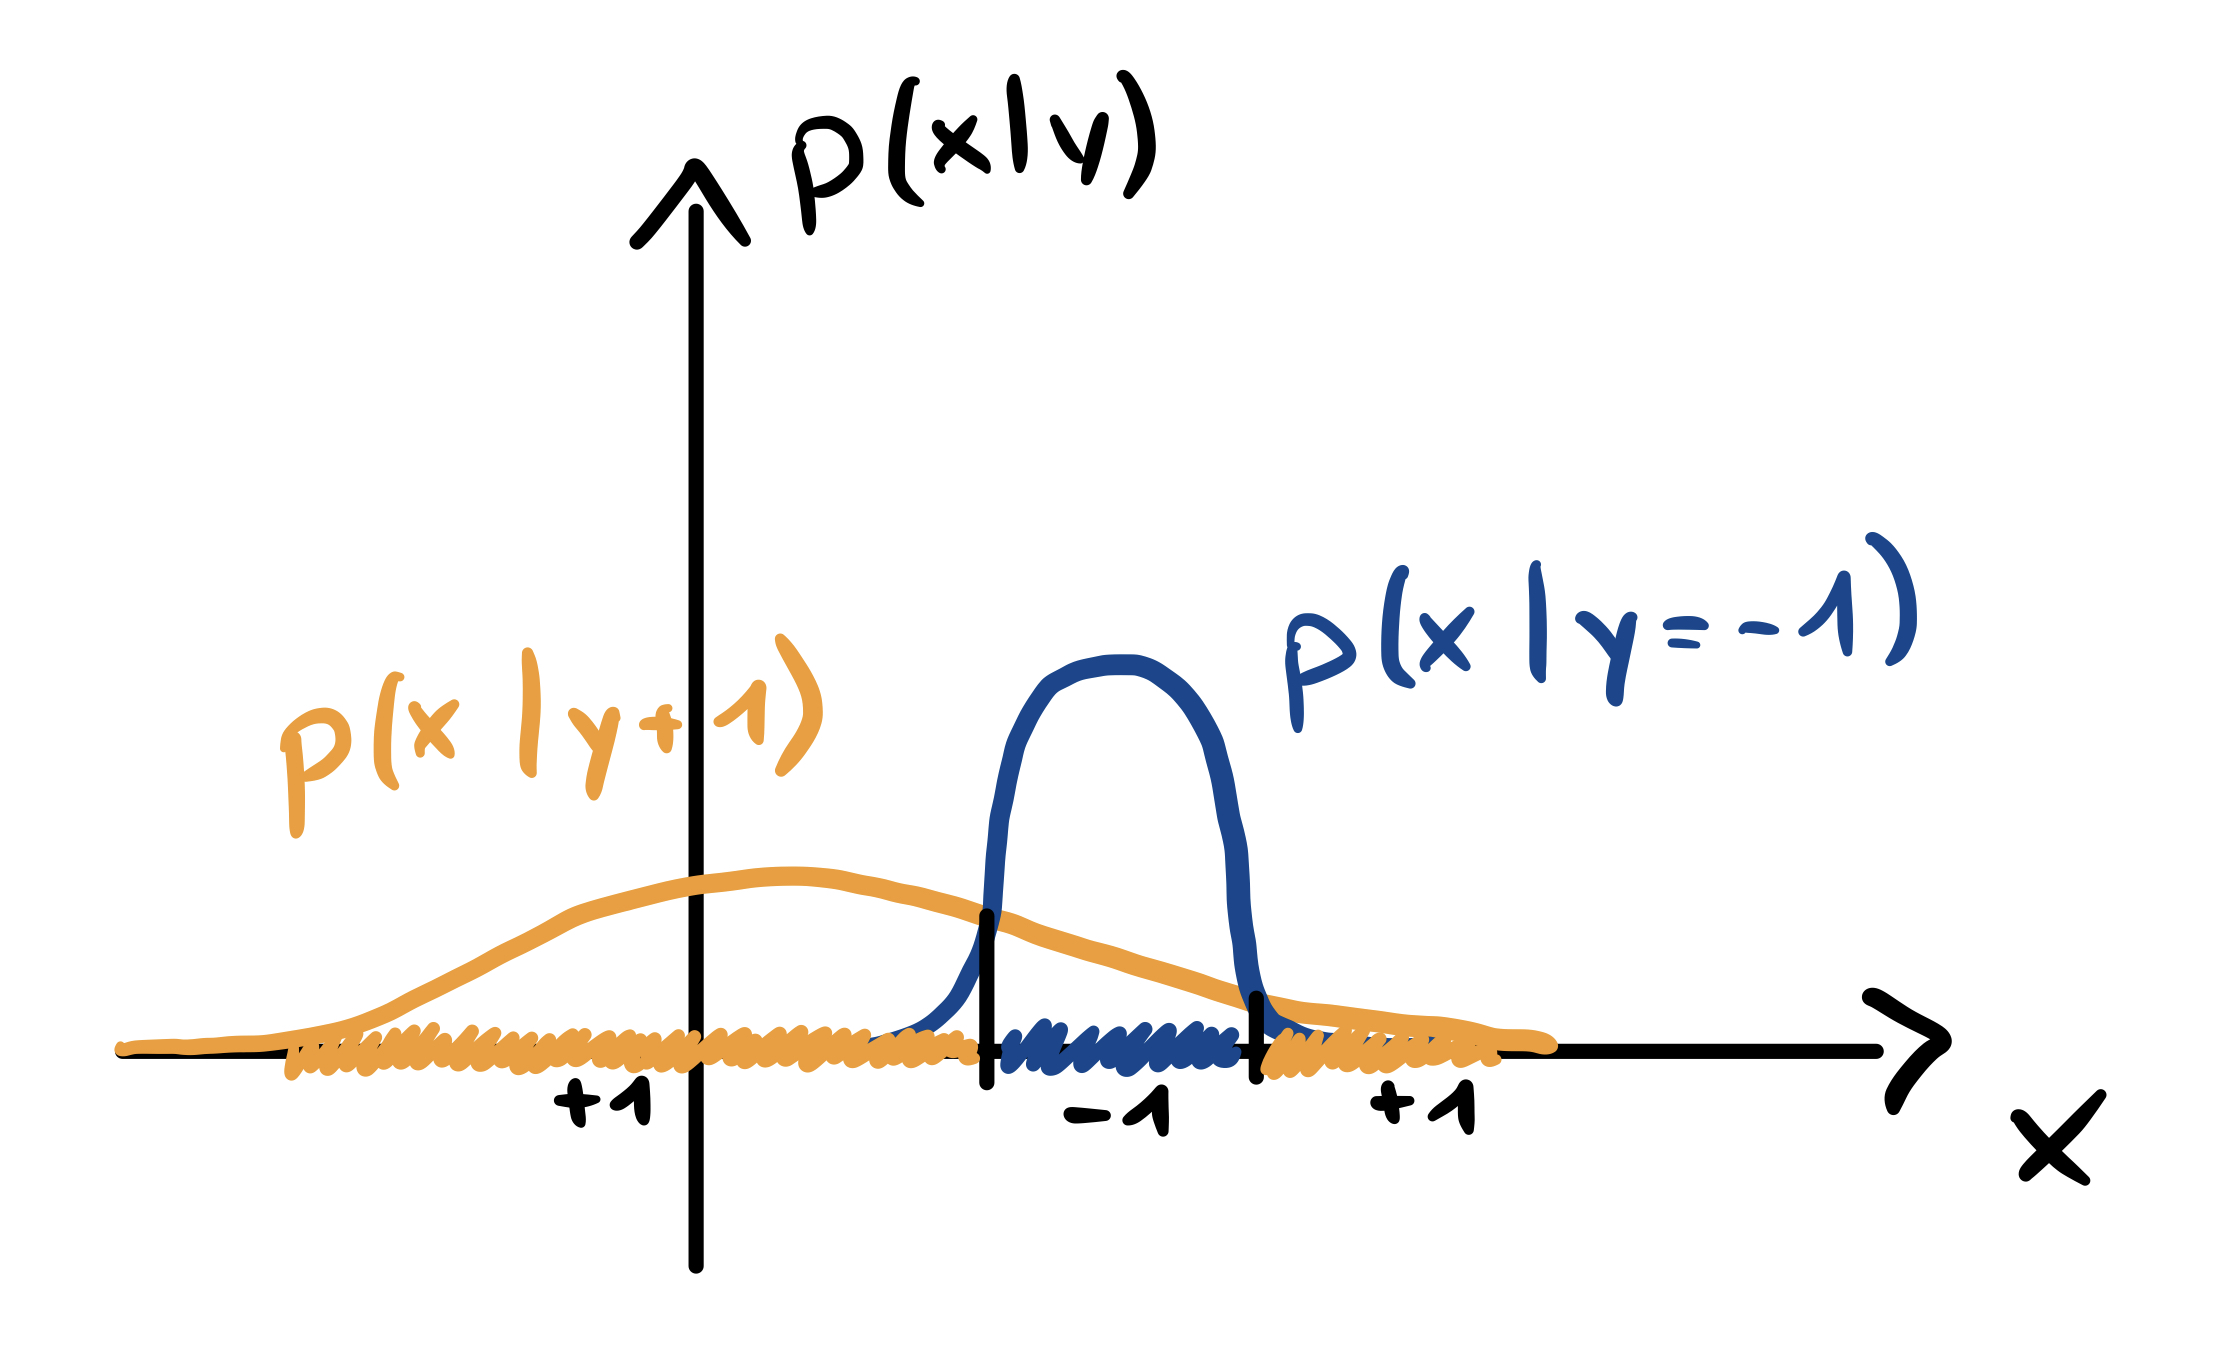
\includegraphics[width=0.8\columnwidth]{gnb.jpeg}
\end{center}

This is equivalent to the following decision rule for binary classification:
$$y = \sgn \underbrace{\left( \log \frac{p(Y = +1 \; | \; x)}{p(Y = -1 \; | \; x)} \right)}_{f(x)}$$

Where $f(x)$ is called the discriminant function. We can rewrite this and get:
\begin{align*}
f(x) &= \sum_{i=1}^d \underbrace{\frac{1}{\sigma_i^2} (\mu_{+1,i} - \mu_{-1,i})}_{w_i} \cdot x_i \\
&+ \underbrace{\log \frac{p}{1-p} + \sum_{i=1}^d \frac{1}{2 \sigma_i^2} (\mu_{-1, i}^2 - \mu_{+1, i}^2)}_{w_0}
\end{align*}

If the conditional independence assumption is violated, we can run into some serious issues, e.g. the classifier can become overconfident.

\subsubsection{Gaussian Bayes Classifier}

We drop the independence assumption and model our features as generated by a multivariant Gaussian $\mathcal{N}(x; \mu_y, \Sigma_y)$ with:
\begin{align*}
	\mu_{y} &= \frac{1}{\text{Count}(Y = y)} \sum_{j \; | \; y_j = y} x_{j}\\
	\Sigma_{y} &= \frac{1}{\text{Count}(Y = y)} \sum_{j \; | \; y_j = y} (x_{j} - \hat \mu_{y}) (x_{j} - \hat \mu_{y})^\top
\end{align*}

This is also called the \textbf{quadratic discriminant analysis} (QDA). If we impose the restriction that $\Sigma_+ = \Sigma_-$ this leads us to the linear discriminant analysis $LDA$ and if we further restrict $p(y) = \frac{1}{2}$ we get the Fisher LDA.

\begin{center}
	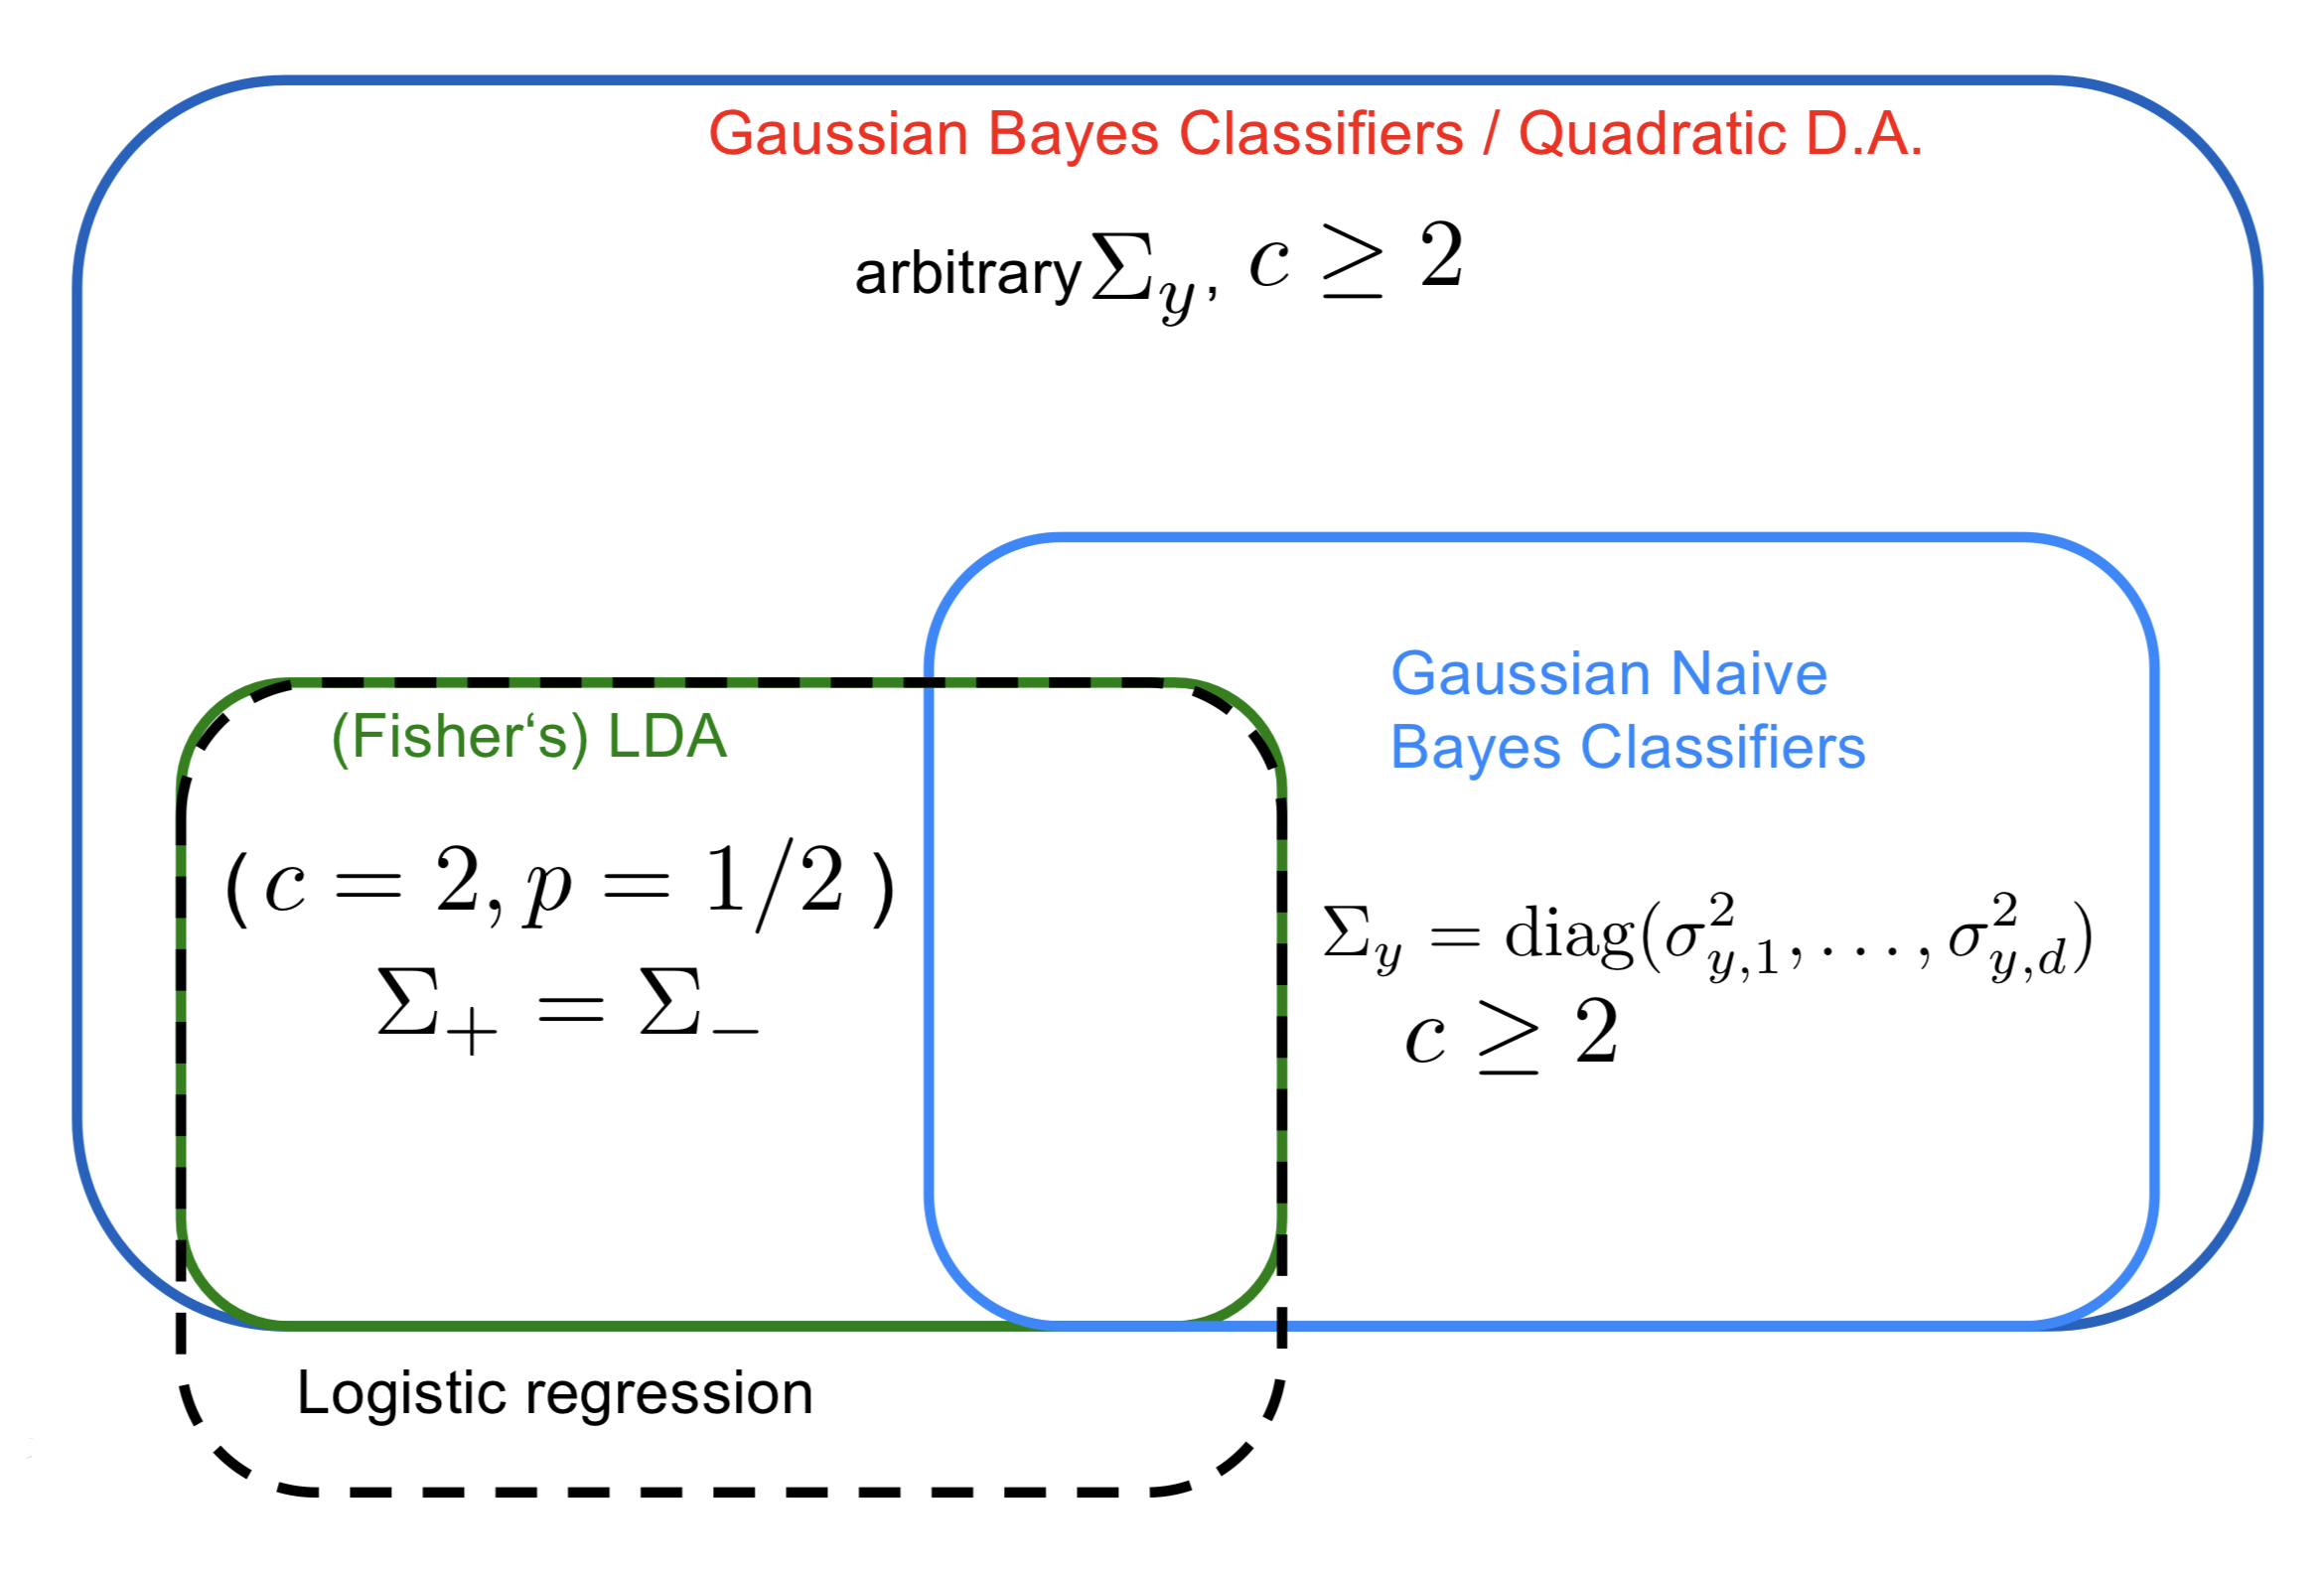
\includegraphics[width=\columnwidth]{qda-bigpicture.jpeg}
\end{center}


